% !TeX program = lualatex
% !TeX encoding = utf8
% !TeX spellcheck = uk_UA
% !BIB program = bibler

\documentclass{beamer}
\usetheme{Electromagnetism}
\usepackage{Electromagnetism}
\hypersetup{
  colorlinks=true,
  linkcolor=cyan,  % Цвет для внутренних ссылок
  urlcolor=red,    % Цвет для URL
  citecolor=blue   % Цвет для библиографических ссылок
}




%============================================================================
\title[Лекції електрики та магнетизму]{\huge\bfseries Магнітне поле у вакуумі}
\subtitle{Лекції з електрики та магнетизму}
\author{Пономаренко С. М.}
\date{}
%============================================================================
\graphicspath{{pictures/}}
\begin{document}


\begin{frame}[plain]
	\maketitle
	%	\tikz[remember picture,overlay] \node[opacity=0.7,inner sep=0pt,
	%		anchor=north west] at (current page.north
	%	west){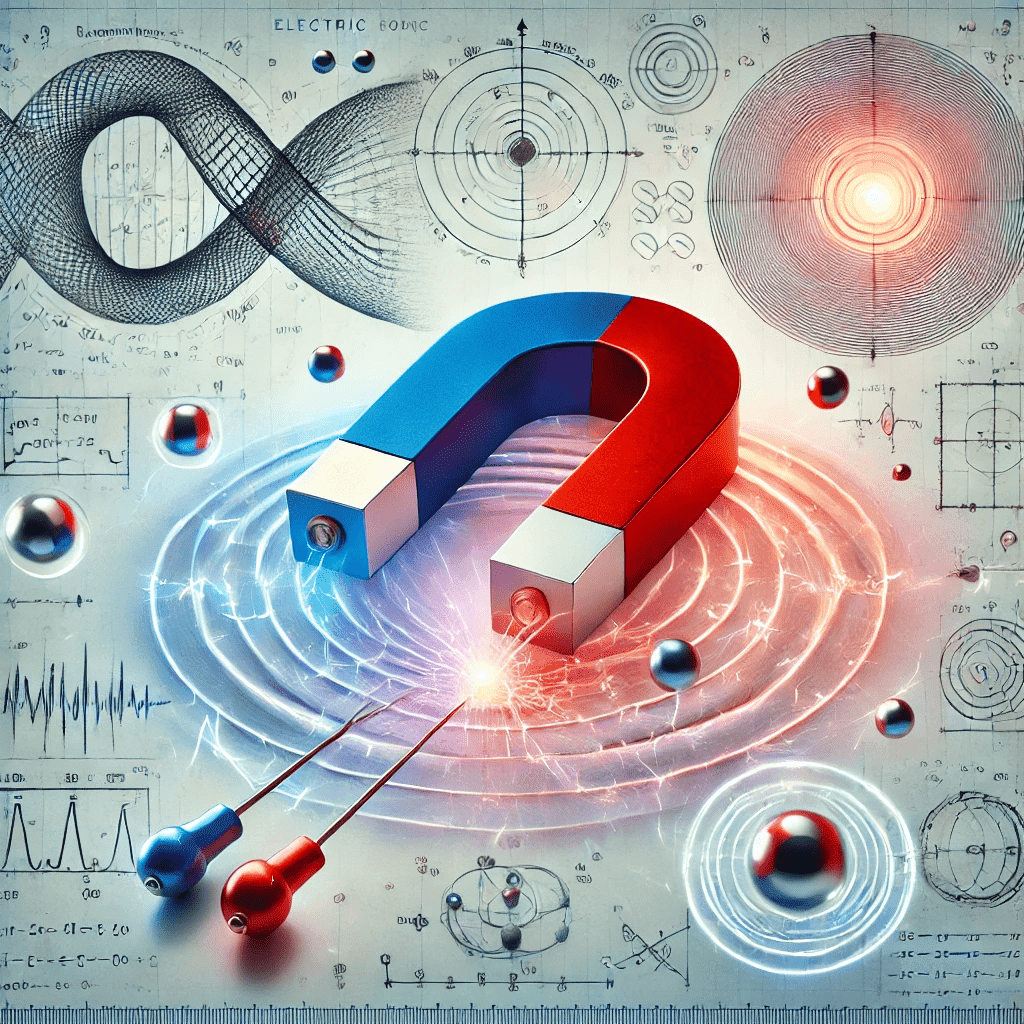
\includegraphics[width=2cm]{EMInteractions}};
\end{frame}

% ============================== Слайд ## ===================================
\begin{frame}{Зміст лекції}{}
	\tableofcontents
\end{frame}
% ===========================================================================

% ============================== Слайд ## ===================================
\begin{frame}{Означення}{}
	\begin{block}{}\justifying
		\alert{Магнітним полем} називається силове поле, що \alert{діє на рухомі заряди} і як наслідок --- на електричні струми  і на тіла, які мають
		магнітний  момент.

		\bigskip

		Магнітне поле створюється рухомими зарядами (електричним струмом). Незмінні в часі струми створюють постійні магнітні поля.
	\end{block}
\end{frame}
% ===========================================================================

% ============================== Слайд ## ===================================
\begin{frame}{Характеристика магнітного поля}{}\small
	\begin{block}{}\justifying
		Магнітних зарядів (магнітних монополів) у в природі немає (експериментальний факт). Характеристику магнітного поля, аналогічно до $\Efield =
			\frac{\vect{F}}{q}$
		ввести не можна. Однак в природі є магнітні диполі (магнітна стрілка, коловий виток зі струмом тощо), тому використовуючи аналогію з моментом
		сил, що діє на електричний диполь в електричному полі $ \vect{M} = \left[\vect{p}_e \times\Efield\right] $, можна ввести характеристику
		магнітного поля:
		\begin{equation*}
			\vect{M} = \left[\vect{p}_m \times\Bfield\right], \quad M_{\max} = p_m B
		\end{equation*}
		Характеристику магнітного поля, вектор $\Bfield$, по історичним причинам називають не \alert{напруженістю}, а \alert{індукцією} магнітного поля.
	\end{block}
	\begin{overprint}
		\onslide<1>
		\begin{block}{}\justifying
			Величина вектора індукції чисельно дорівнює максимальному обертальному моменту, що діє на одиничний магнітний момент вміщений у магнітне поле:
			\begin{equation*}
				B = \frac{\quad M_{\max}}{p_m}.
			\end{equation*}
		\end{block}
		\onslide<2>
		\begin{alertblock}{}\justifying
			В гауссовій системі одиниць величину магнітного поля називають Гаусом (Гс). С системі СІ Теслою (Тл):
			\begin{equation*}
				1\ \text{Тл} = 10^4\ \text{Гс}.
			\end{equation*}
		\end{alertblock}
	\end{overprint}
\end{frame}
% ===========================================================================

% ============================== Слайд ## ===================================
\begin{frame}{Сила Лоренца та сила Ампера}{}
	\begin{block}{}
		Магнітною складовою сили Лоренца називається сила, що діє на рухомий заряд $q$ з боку магнітного поля:
		\begin{equation*}
			\vect{F} = q\left[\frac{\vect{v}}{c}\times\Bfield\right].
		\end{equation*}
		Повна сила (власне і є сила Лоренца), що діє на заряд, включає також силу з боку електричного поля:
		\begin{equation*}
			\vect{F} = q\left( \Efield + \left[\frac{\vect{v}}{c}\times\Bfield\right] \right) .
		\end{equation*}
	\end{block}
	\begin{block}{}
		\alert{Силою Ампера} називають силу, що діє на струми з боку магнітного поля:
		\begin{equation*}
			d\vect{F} = \frac1c \left[ \vect{j}dV \times \Bfield\right],
		\end{equation*}
		де $\vect{j} dV$ --- називається об'ємним \alert{елементом струму}, а добуток $Id\vect{\ell}$ --- лінійним елементом струму.
	\end{block}
\end{frame}
% ===========================================================================


% ============================== Слайд ## ===================================
\begin{frame}{Зв'язок сили Лоренца та сили Ампера}{}
	\begin{block}{}
		Сила Лоренца, що діє на заряд $dq$, дорівнює
		\begin{equation*}
			\vect{F} = \left[\frac{dq \vect{v}}{c}\times\Bfield\right].
		\end{equation*}
		Оскільки $dq \vect{v} = \rho \vect{v} dV = \vect{j} dV$, то одразу отримуємо силу Ампера, що діє на об'ємний елемент струму:
		\begin{equation*}
			d\vect{F} = \frac1c \left[ \vect{j}dV \times \Bfield\right].
		\end{equation*}
	\end{block}
\end{frame}
% ===========================================================================



% ============================== Слайд ## ===================================
\begin{frame}{Закон Біо-Савара-Лапласа}{}
	\begin{block}{}\justifying
		Закон Біо-Савара встановлено експериментально (1820 р.) шляхом аналізу експериментальних даних і \alert{визначає магнітне поле, що створюється
			елементом струму}.
	\end{block}
\end{frame}
% ===========================================================================

\end{document}
